\documentclass[10pt,landscape]{article}
\usepackage[a0paper,margin=2in]{geometry}

\usepackage{graphicx}
\usepackage{epstopdf}
\usepackage{xcolor}

\definecolor{pastel_1}{HTML}{FAB3AE}
\definecolor{pastel_2}{HTML}{B3CFE3}
\definecolor{pastel_3}{HTML}{CCEBC5}
\definecolor{pastel_4}{HTML}{DECAE3}
\definecolor{pastel_5}{HTML}{FDD7A6}
\definecolor{pastel_6}{HTML}{FFFDCC}
\definecolor{pastel_7}{HTML}{E3D7BD}

\begin{document}
\pagenumbering{gobble}

\hspace{0.1\linewidth}
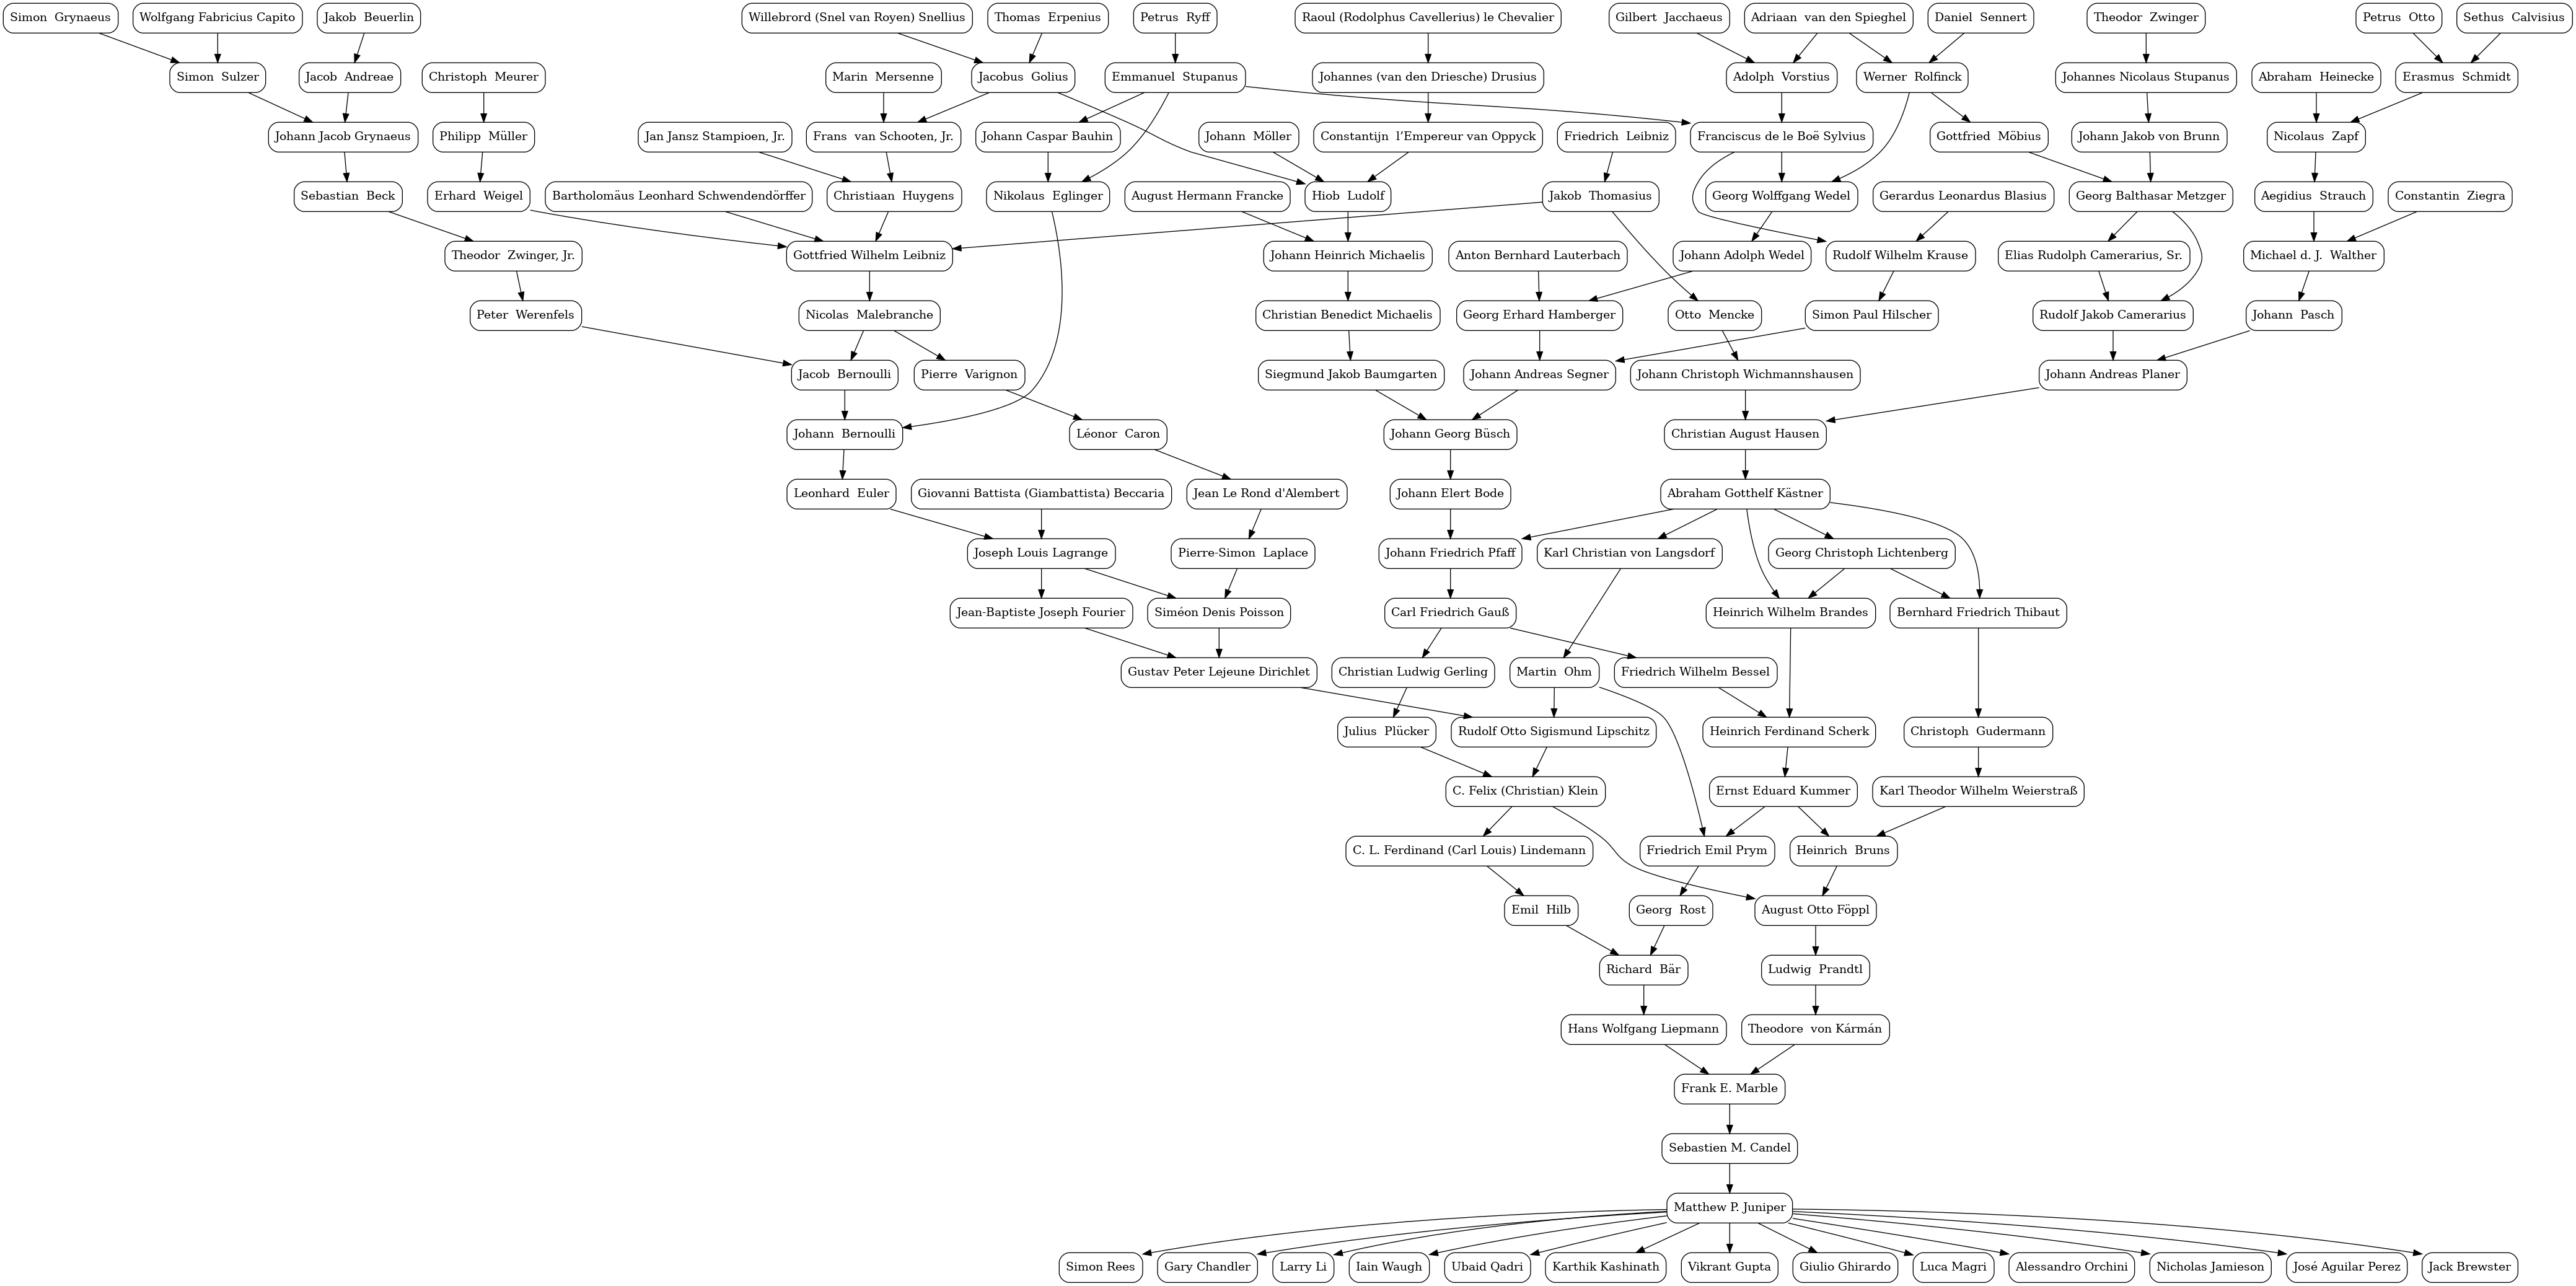
\includegraphics[width=0.75\linewidth]{juniper.eps}
\hspace{-0.05\linewidth}
\begin{tabular}[b]{|p{0.5cm}p{20cm}p{0.5cm}|}
\hline
&&\\
&&\\
& \centering \Huge \underline{\bf Matthew P.\ Juniper's academic genealogy} & \\
&&\\
&&\\
\begin{tabular}[b]{p{10cm}p{10cm}}
\Huge \textcolor{pastel_1}{\rule{2cm}{0.5cm}} \quad after 2000 & \Huge \textcolor{pastel_5}{\rule{2cm}{0.5cm}} \quad after 1600 \\
&\\
\Huge \textcolor{pastel_2}{\rule{2cm}{0.5cm}} \quad after 1900 & \Huge \textcolor{pastel_6}{\rule{2cm}{0.5cm}} \quad after 1500 \\
&\\
\Huge \textcolor{pastel_3}{\rule{2cm}{0.5cm}} \quad after 1800 & \Huge \textcolor{pastel_7}{\rule{2cm}{0.5cm}} \quad after 1400 \\
&\\
\Huge \textcolor{pastel_4}{\rule{2cm}{0.5cm}} \quad after 1700 & \\
\end{tabular}
&&\\
&&\\
\hline
\end{tabular}

\end{document}
